\documentclass[border=10pt]{standalone}
\usepackage{tikz}
\usetikzlibrary{shapes,arrows,positioning}

\begin{document}
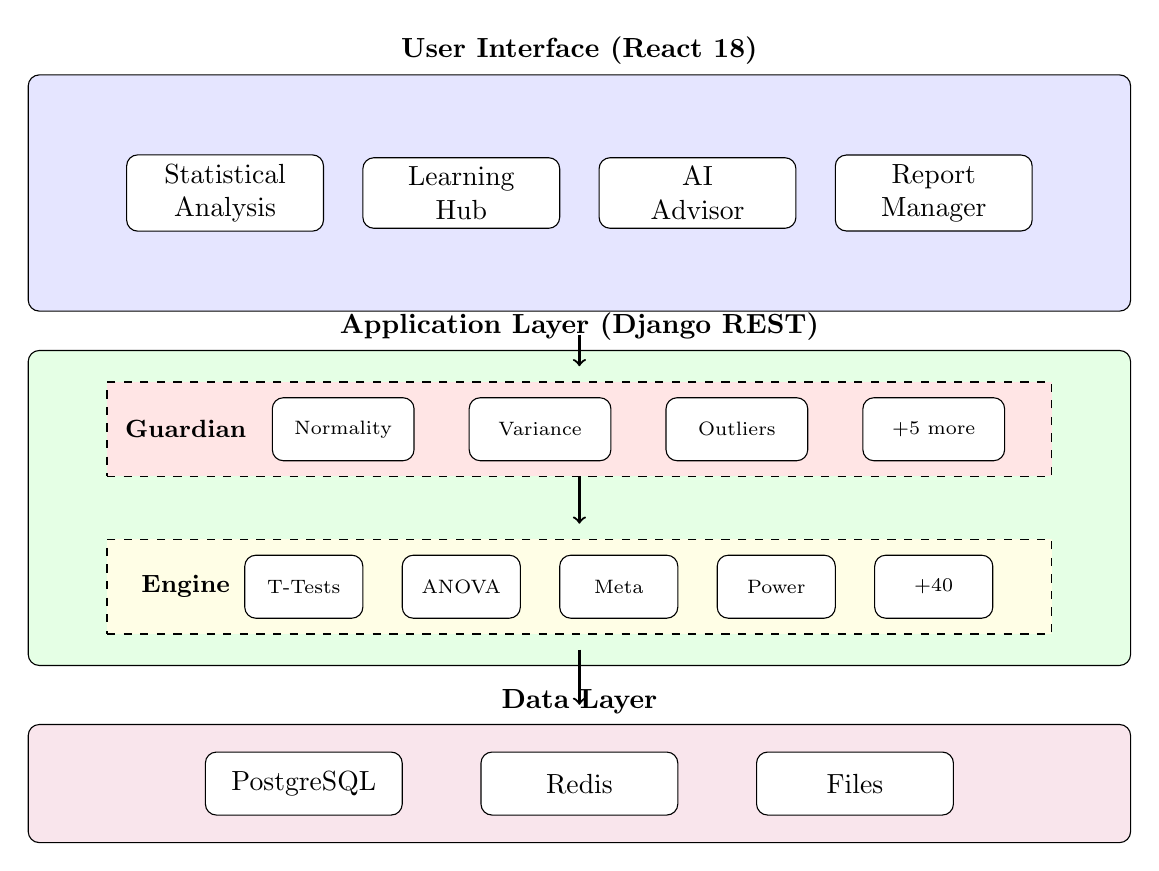
\begin{tikzpicture}[
    box/.style={draw, rounded corners, minimum width=2.5cm, minimum height=0.8cm, align=center},
    layer/.style={draw, rounded corners, minimum width=14cm, minimum height=2cm, fill=gray!10},
    arrow/.style={->, thick}
]

% User Interface Layer
\node[layer, minimum height=3cm, fill=blue!10] (ui) at (0,6) {};
\node[above] at (ui.north) {\textbf{User Interface (React 18)}};
\node[box, fill=white] at (-4.5,6) {Statistical\\Analysis};
\node[box, fill=white] at (-1.5,6) {Learning\\Hub};
\node[box, fill=white] at (1.5,6) {AI\\Advisor};
\node[box, fill=white] at (4.5,6) {Report\\Manager};

% Application Layer
\node[layer, minimum height=4cm, fill=green!10] (app) at (0,2) {};
\node[above] at (app.north) {\textbf{Application Layer (Django REST)}};

% Guardian sublayer
\node[draw, dashed, minimum width=12cm, minimum height=1.2cm, fill=red!10] at (0,3) {};
\node at (-5,3) {\small\textbf{Guardian}};
\node[box, fill=white, minimum width=1.8cm, font=\scriptsize] at (-3,3) {Normality};
\node[box, fill=white, minimum width=1.8cm, font=\scriptsize] at (-0.5,3) {Variance};
\node[box, fill=white, minimum width=1.8cm, font=\scriptsize] at (2,3) {Outliers};
\node[box, fill=white, minimum width=1.8cm, font=\scriptsize] at (4.5,3) {+5 more};

% Statistical Engine
\node[draw, dashed, minimum width=12cm, minimum height=1.2cm, fill=yellow!10] at (0,1) {};
\node at (-5,1) {\small\textbf{Engine}};
\node[box, fill=white, minimum width=1.5cm, font=\scriptsize] at (-3.5,1) {T-Tests};
\node[box, fill=white, minimum width=1.5cm, font=\scriptsize] at (-1.5,1) {ANOVA};
\node[box, fill=white, minimum width=1.5cm, font=\scriptsize] at (0.5,1) {Meta};
\node[box, fill=white, minimum width=1.5cm, font=\scriptsize] at (2.5,1) {Power};
\node[box, fill=white, minimum width=1.5cm, font=\scriptsize] at (4.5,1) {+40};

% Data Layer
\node[layer, minimum height=1.5cm, fill=purple!10] (data) at (0,-1.5) {};
\node[above] at (data.north) {\textbf{Data Layer}};
\node[box, fill=white] at (-3.5,-1.5) {PostgreSQL};
\node[box, fill=white] at (0,-1.5) {Redis};
\node[box, fill=white] at (3.5,-1.5) {Files};

% Arrows
\draw[arrow] (0,4.2) -- (0,3.8);
\draw[arrow] (0,2.4) -- (0,1.8);
\draw[arrow] (0,0.2) -- (0,-0.5);

\end{tikzpicture}
\end{document}
